% Options for packages loaded elsewhere
% Options for packages loaded elsewhere
\PassOptionsToPackage{unicode}{hyperref}
\PassOptionsToPackage{hyphens}{url}
\PassOptionsToPackage{dvipsnames,svgnames,x11names}{xcolor}
%
\documentclass[
  british,
  a4paper,
]{article}
\usepackage{xcolor}
\usepackage{amsmath,amssymb}
\setcounter{secnumdepth}{-\maxdimen} % remove section numbering
\usepackage{iftex}
\ifPDFTeX
  \usepackage[T1]{fontenc}
  \usepackage[utf8]{inputenc}
  \usepackage{textcomp} % provide euro and other symbols
\else % if luatex or xetex
  \usepackage{unicode-math} % this also loads fontspec
  \defaultfontfeatures{Scale=MatchLowercase}
  \defaultfontfeatures[\rmfamily]{Ligatures=TeX,Scale=1}
\fi
\usepackage{lmodern}
\ifPDFTeX\else
  % xetex/luatex font selection
\fi
% Use upquote if available, for straight quotes in verbatim environments
\IfFileExists{upquote.sty}{\usepackage{upquote}}{}
\IfFileExists{microtype.sty}{% use microtype if available
  \usepackage[]{microtype}
  \UseMicrotypeSet[protrusion]{basicmath} % disable protrusion for tt fonts
}{}
\makeatletter
\@ifundefined{KOMAClassName}{% if non-KOMA class
  \IfFileExists{parskip.sty}{%
    \usepackage{parskip}
  }{% else
    \setlength{\parindent}{0pt}
    \setlength{\parskip}{6pt plus 2pt minus 1pt}}
}{% if KOMA class
  \KOMAoptions{parskip=half}}
\makeatother
% Make \paragraph and \subparagraph free-standing
\makeatletter
\ifx\paragraph\undefined\else
  \let\oldparagraph\paragraph
  \renewcommand{\paragraph}{
    \@ifstar
      \xxxParagraphStar
      \xxxParagraphNoStar
  }
  \newcommand{\xxxParagraphStar}[1]{\oldparagraph*{#1}\mbox{}}
  \newcommand{\xxxParagraphNoStar}[1]{\oldparagraph{#1}\mbox{}}
\fi
\ifx\subparagraph\undefined\else
  \let\oldsubparagraph\subparagraph
  \renewcommand{\subparagraph}{
    \@ifstar
      \xxxSubParagraphStar
      \xxxSubParagraphNoStar
  }
  \newcommand{\xxxSubParagraphStar}[1]{\oldsubparagraph*{#1}\mbox{}}
  \newcommand{\xxxSubParagraphNoStar}[1]{\oldsubparagraph{#1}\mbox{}}
\fi
\makeatother


\usepackage{longtable,booktabs,array}
\newcounter{none} % for unnumbered tables
\usepackage{calc} % for calculating minipage widths
% Correct order of tables after \paragraph or \subparagraph
\usepackage{etoolbox}
\makeatletter
\patchcmd\longtable{\par}{\if@noskipsec\mbox{}\fi\par}{}{}
\makeatother
% Allow footnotes in longtable head/foot
\IfFileExists{footnotehyper.sty}{\usepackage{footnotehyper}}{\usepackage{footnote}}
\makesavenoteenv{longtable}
\usepackage{graphicx}
\makeatletter
\newsavebox\pandoc@box
\newcommand*\pandocbounded[1]{% scales image to fit in text height/width
  \sbox\pandoc@box{#1}%
  \Gscale@div\@tempa{\textheight}{\dimexpr\ht\pandoc@box+\dp\pandoc@box\relax}%
  \Gscale@div\@tempb{\linewidth}{\wd\pandoc@box}%
  \ifdim\@tempb\p@<\@tempa\p@\let\@tempa\@tempb\fi% select the smaller of both
  \ifdim\@tempa\p@<\p@\scalebox{\@tempa}{\usebox\pandoc@box}%
  \else\usebox{\pandoc@box}%
  \fi%
}
% Set default figure placement to htbp
\def\fps@figure{htbp}
\makeatother



\ifLuaTeX
\usepackage[bidi=basic,shorthands=off]{babel}
\else
\usepackage[bidi=default,shorthands=off]{babel}
\fi
\ifLuaTeX
  \usepackage{selnolig} % disable illegal ligatures
\fi


\setlength{\emergencystretch}{3em} % prevent overfull lines

\providecommand{\tightlist}{%
  \setlength{\itemsep}{0pt}\setlength{\parskip}{0pt}}



 


\makeatletter
\@ifpackageloaded{tcolorbox}{}{\usepackage[skins,breakable]{tcolorbox}}
\@ifpackageloaded{fontawesome5}{}{\usepackage{fontawesome5}}
\definecolor{quarto-callout-color}{HTML}{909090}
\definecolor{quarto-callout-note-color}{HTML}{0758E5}
\definecolor{quarto-callout-important-color}{HTML}{CC1914}
\definecolor{quarto-callout-warning-color}{HTML}{EB9113}
\definecolor{quarto-callout-tip-color}{HTML}{00A047}
\definecolor{quarto-callout-caution-color}{HTML}{FC5300}
\definecolor{quarto-callout-color-frame}{HTML}{acacac}
\definecolor{quarto-callout-note-color-frame}{HTML}{4582ec}
\definecolor{quarto-callout-important-color-frame}{HTML}{d9534f}
\definecolor{quarto-callout-warning-color-frame}{HTML}{f0ad4e}
\definecolor{quarto-callout-tip-color-frame}{HTML}{02b875}
\definecolor{quarto-callout-caution-color-frame}{HTML}{fd7e14}
\makeatother
\makeatletter
\@ifpackageloaded{caption}{}{\usepackage{caption}}
\AtBeginDocument{%
\ifdefined\contentsname
  \renewcommand*\contentsname{Table of contents}
\else
  \newcommand\contentsname{Table of contents}
\fi
\ifdefined\listfigurename
  \renewcommand*\listfigurename{List of Figures}
\else
  \newcommand\listfigurename{List of Figures}
\fi
\ifdefined\listtablename
  \renewcommand*\listtablename{List of Tables}
\else
  \newcommand\listtablename{List of Tables}
\fi
\ifdefined\figurename
  \renewcommand*\figurename{Figure}
\else
  \newcommand\figurename{Figure}
\fi
\ifdefined\tablename
  \renewcommand*\tablename{Table}
\else
  \newcommand\tablename{Table}
\fi
}
\@ifpackageloaded{float}{}{\usepackage{float}}
\floatstyle{ruled}
\@ifundefined{c@chapter}{\newfloat{codelisting}{h}{lop}}{\newfloat{codelisting}{h}{lop}[chapter]}
\floatname{codelisting}{Listing}
\newcommand*\listoflistings{\listof{codelisting}{List of Listings}}
\makeatother
\makeatletter
\makeatother
\makeatletter
\@ifpackageloaded{caption}{}{\usepackage{caption}}
\@ifpackageloaded{subcaption}{}{\usepackage{subcaption}}
\makeatother
\usepackage{bookmark}
\IfFileExists{xurl.sty}{\usepackage{xurl}}{} % add URL line breaks if available
\urlstyle{same}
% fallback for those not using the hyperref driver hyperxmp:
\makeatletter
\@ifundefined{xmpquote}{\newcommand{\xmpquote}[1]{#1}}{}
\makeatother
\hypersetup{
  pdftitle={Was Mexico really more productive than the US in 1980?},
  pdfauthor={Carlos Galindo},
  pdflang={en-GB},
  colorlinks=true,
  linkcolor={blue},
  filecolor={Maroon},
  citecolor={Blue},
  urlcolor={Blue},
  pdfcreator={LaTeX via pandoc}}


\title{Was Mexico really more productive than the US in 1980?}
\usepackage{etoolbox}
\makeatletter
\providecommand{\subtitle}[1]{% add subtitle to \maketitle
  \apptocmd{\@title}{\par {\large #1 \par}}{}{}
}
\makeatother
\subtitle{A puzzle in the standard cross-country productivity data turns
out to be mostly a price-comparison artefact}
\author{Carlos Galindo}
\date{}
\begin{document}
\maketitle


\begin{tcolorbox}[enhanced jigsaw, arc=.35mm, bottomrule=.15mm, breakable, colback=white, colframe=quarto-callout-note-color-frame, left=2mm, leftrule=.75mm, opacityback=0, rightrule=.15mm, toprule=.15mm]

\vspace{-3mm}\textbf{At a glance}\vspace{3mm}

\begin{itemize}
\tightlist
\item
  \textbf{Question.} Why does the Penn World Table show Mexico's total
  factor productivity above the US level in 1980 and 1981, when Mexican
  income per head was about half the US level?
\item
  \textbf{Approach.} Check the capital-share assumption, break aggregate
  productivity into sectors, isolate the oil boom, and test whether the
  price deflators behind purchasing-power comparisons can generate the
  gap.
\item
  \textbf{Finding.} The gap is mostly a measurement artefact of the
  deflators used for purchasing-power comparisons, with smaller real
  contributions from the oil boom and from Mexico's high measured
  capital share.
\item
  \textbf{Why it matters.} Taken at face value, the data tell a story of
  a collapse from leader to laggard. Corrected, they describe a country
  that never closed the gap at all.
\end{itemize}

\end{tcolorbox}

\subsection{The question}\label{the-question}

Total factor productivity (TFP) is the part of output that capital and
labour do not explain. It is the usual measure of how efficiently an
economy turns inputs into output, and it is the number behind many
growth narratives. Cross-country comparisons of it rest on one input
above all: a way to value output in a common currency. That is the job
of purchasing-power price comparisons.

The Penn World Table, in its latest edition, contains a result that
should stop any economist. On its aggregate TFP measure, scaled so that
the US in 2019 equals 1.0, Mexico stands at 1.51 against a US value held
at 1.00 in 1980, and 1.50 in 1981. In the same years, Mexican real
income per head was roughly half the US level. A country is being
described as 51 per cent more efficient than the richest large economy
while being about 52 per cent poorer.

There are two ways to read this. One is to take it as a fact and build a
story on it: Mexico was a productivity leader in 1980 and then lost its
edge. The other is to ask whether the number is measuring what we think
it is. This note follows the second route. The question matters because
a growth narrative resting on a spurious starting point misdiagnoses
everything that follows, including how large the later decline was and
what would be needed to reverse it.

\subsection{Approach}\label{approach}

The investigation had four steps, each designed to eliminate one
explanation before moving to the next.

\textbf{First, the capital share.} Standard TFP calculations weight
capital and labour by factor shares. Mexico's measured capital share in
1980 was far higher than the US share, 0.605 against 0.376. A high
capital share changes how much of output is attributed to inputs and how
much is left as TFP, so it is the first candidate for a mechanical
distortion. The test is simple: recompute productivity for both
countries with a single common capital share of one third, and see
whether the gap closes.

\textbf{Second, a sectoral breakdown.} Aggregate productivity hides
where it comes from. A sectoral database of value added and employment
for the major sectors of each economy allows productivity per worker to
be compared sector by sector, in constant prices converted to a common
currency. If Mexico really were more efficient, the advantage should be
concentrated in a few places, and it should be plausible in each of
them.

\textbf{Third, the oil boom.} Mexico's oil sector expanded sharply in
the late 1970s as oil prices rose. Mining and oil employed only a small
share of the workforce but produced very high output per worker. The
question is how much of the aggregate gap that single sector can carry.
A shift-share style decomposition, which splits changes in aggregate
productivity into within-sector and between-sector parts, was also used
to check the plausibility of the sector series. An early version
produced absurd growth figures because nominal rather than constant
prices had been used; catching that against a simple cross-check on
employment shares was part of the validation.

\textbf{Fourth, the deflators.} The comparison of sectoral output across
countries relies on price indices and purchasing-power conversion
factors that are defined for the whole economy, not for each sector. If
those aggregate factors misvalue a sector's output, productivity in that
sector will be misstated by the same proportion. The test here is one of
plausibility: do the implied sector ratios make economic sense?

The data are the Penn World Table (aggregate TFP, capital shares,
income) and a sectoral productivity database covering ten sectors. The
work compares a developing and a rich economy, 1975--1985 for the
paradox itself.

\subsection{What the work shows}\label{what-the-work-shows}

\textbf{The paradox is stable, not a one-year blip.} The published ratio
of Mexican to US TFP was 1.27 in 1975, 1.51 in 1980, 1.50 in 1981 and
1.20 in 1985. It rises with the oil boom and falls after it, but stays
above one throughout, while the income ratio stays well below one (0.45,
0.48, 0.50 and 0.42 in the same years).

\begin{figure}

\centering{

\pandocbounded{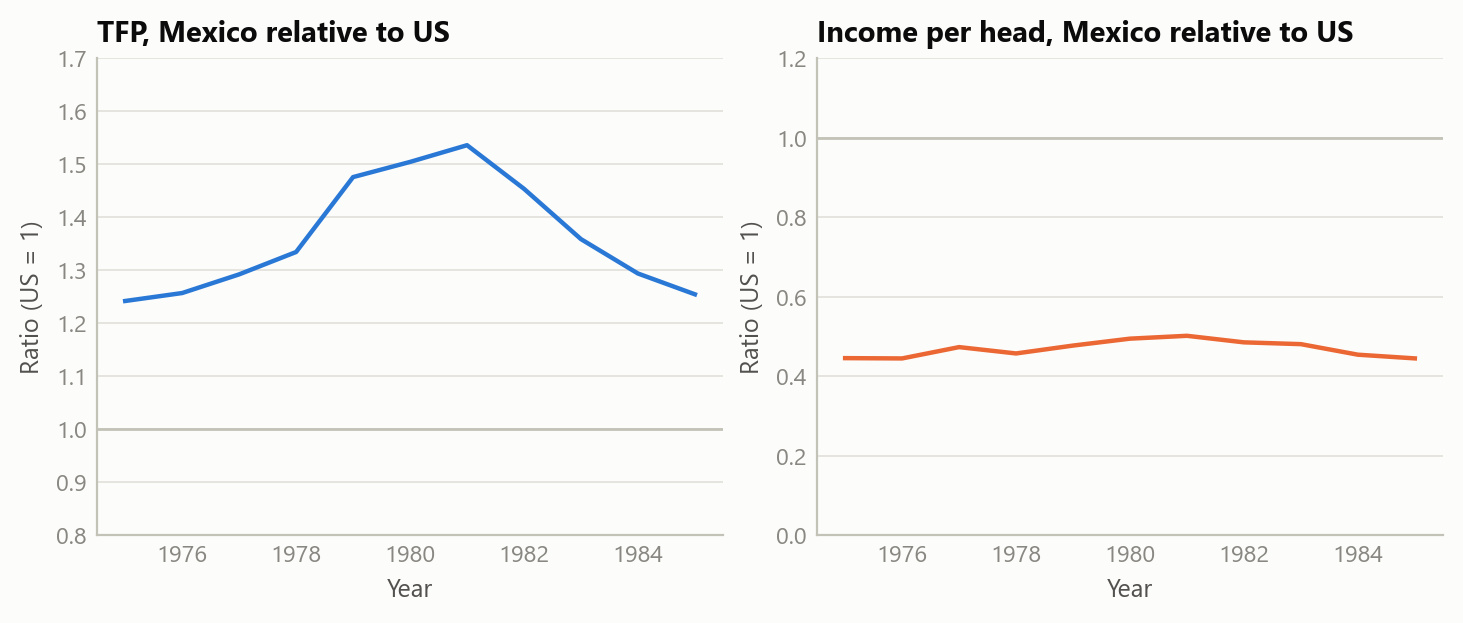
\includegraphics[keepaspectratio]{index_files/figure-latex/fig-paradox-output-1.png}}

}

\caption{\label{fig-paradox}Stylised version of the puzzle: a TFP ratio
above one alongside an income ratio below one, 1975--1985 (simulated
data).}

\end{figure}%

\textbf{Fixing the capital share does not remove it.} With a common
capital share, the Mexican advantage falls to 24 per cent in 1980 and 27
per cent in 1981 --- smaller, but still there. The capital-share
difference is a real, mechanical contributor, and the investigation put
it at roughly a fifth of the paradox. It does not explain the rest.

\textbf{The advantage is implausibly broad.} In 1980, labour
productivity outside agriculture was about 4.7 times higher in Mexico
than in the US on the sectoral data, and every non-agricultural sector
showed a Mexican lead. The ratios ran from 1.5 times in personal
services to 12.3 times in trade services, 8.0 times in business services
and 5.4 times in manufacturing. Few of these can be believed. A Mexican
retail worker is not twelve times as productive as a US one, and Mexican
factories were not five times as productive as US factories at a time
when the US led in automation, management practice and skills.

\begin{figure}

\centering{

\pandocbounded{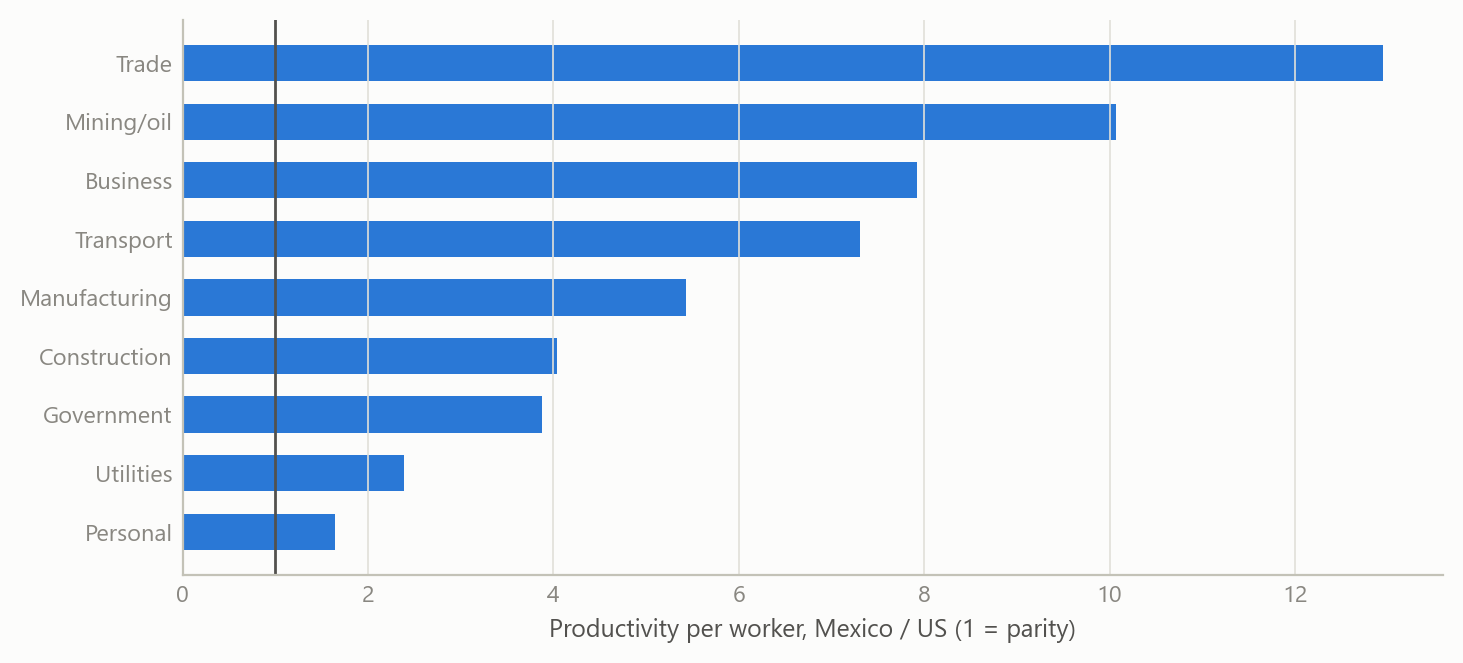
\includegraphics[keepaspectratio]{index_files/figure-latex/fig-sectors-output-1.png}}

}

\caption{\label{fig-sectors}Stylised sectoral productivity ratios,
Mexico relative to US (simulated data).}

\end{figure}%

\textbf{The oil boom is real but small.} Mining and oil employed about
1.4 per cent of Mexican workers in 1980, yet output per worker was about
10.3 times the US figure, and 14.3 times in 1981. Real in this case
means a genuine resource-price windfall, not a mismeasurement. But a
sector that small can carry only a small part of an aggregate gap: the
investigation estimated roughly 8 per cent of it.

\textbf{Most of what remains is the price comparison.} The sectoral
series convert output with deflators and purchasing-power factors
defined for the aggregate economy. They do not adjust sector by sector,
and they do not adjust for quality: an output of the same nominal value
in Mexico and in the US is not the same real quantity when the goods and
services differ in quality and variety. The effect should be largest in
services and in goods where quality differences are widest, which is
exactly where the implausible ratios appear. The investigation
attributed about 70 per cent of the paradox to measurement (roughly 60
per cent to the aggregate deflators and 10 per cent to missing quality
adjustment) and 30 per cent to real factors (about 20 per cent from the
capital share and 10 per cent from oil). On its working estimate,
Mexican TFP in 1980 was about 65 per cent of the US level, not 151 per
cent.

A small simulation makes the mechanism concrete. If the deflator
overstates the real value of Mexican output by a given percentage, the
measured productivity ratio rises one-for-one, and the error compounds
in sectors that dominate employment.

\begin{figure}

\centering{

\pandocbounded{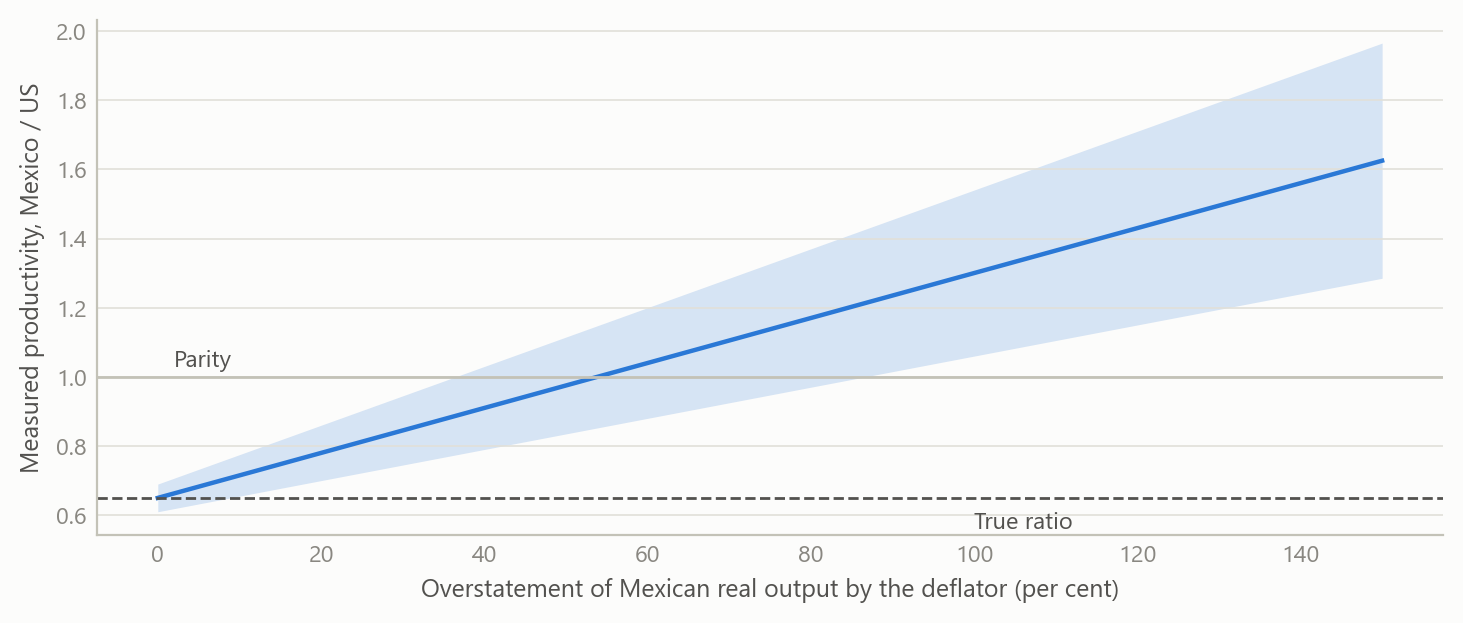
\includegraphics[keepaspectratio]{index_files/figure-latex/fig-deflator-output-1.png}}

}

\caption{\label{fig-deflator}How a deflator error moves the measured
productivity ratio, for a true ratio of 0.65 (simulated data).}

\end{figure}%

\subsection{Insights}\label{insights}

\begin{enumerate}
\def\labelenumi{\arabic{enumi}.}
\tightlist
\item
  \textbf{When a poorer country beats a richer one on productivity,
  suspect the yardstick first.} An efficiency lead alongside half the
  income is not impossible, but it is a prompt to check the measurement
  before building a story on it.
\item
  \textbf{Aggregate price conversions are not sector-specific.} Sectoral
  levels converted with economy-wide factors are good for composition
  and for growth within a sector, and poor for comparing levels across
  countries, particularly in services.
\item
  \textbf{Decompose before you explain.} The aggregate paradox came
  apart into three pieces with different characters: a mechanical one
  (capital share), a real but tiny one (oil) and a large measurement
  one. Each needed a different response.
\item
  \textbf{Resource-rich countries break the standard capital share.} A
  common share of one third is a convenient assumption, but a measured
  share of about 0.6 against 0.38 is large enough to move the answer.
\item
  \textbf{The corrected story is, if anything, harsher.} If Mexico was
  never ahead, the post-1981 decline in the published series is mostly
  an artefact too, and the real finding is persistence: relative
  productivity stayed near 60 to 65 per cent of the US level for
  decades, in spite of heavy capital accumulation and rising schooling.
  The problem is one of never converging, not of losing a lead.
\end{enumerate}

\subsection{Scope and next steps}\label{scope-and-next-steps}

The investigation is built to separate real productivity performance
from measurement in Mexico's record, using sector ratios, plausibility
arguments, and tests on the capital share and the oil sector. Its
attribution of roughly 70 per cent to measurement, and the corrected
productivity level of about 65 per cent of the US, are reasoned
judgements built from those tests.

The natural extensions are two. First, a formal decomposition that nests
the deflator channel as a parameter and attaches confidence intervals to
the attribution. Second, a sector-by-sector re-pricing with detailed
international price survey data in place of aggregate factors, across
more countries and sectors.

\subsection{About the evidence}\label{about-the-evidence}

This note covers a 2025 investigation of published international
productivity data for Mexico and the US around 1980. The numbers in the
text are results of that work. The figures are simulated: they have the
same variables, years and sector structure as the real analysis, and
show the mechanism rather than the published values.

Figures and tables marked \emph{simulated} are generated from simulated
data built to share the structure of the analysis (its variables,
horizons and frequencies). They show how each method works and what its
output looks like. Results stated in the text, and figures that give a
source, are the project's own. Methods are described at the level of a
methods section. Code and data pipelines are not reproduced here.




\end{document}
